\documentclass[conference]{IEEEtran}
\IEEEoverridecommandlockouts

\usepackage{cite}
\usepackage{amsmath,amssymb,amsfonts}
\usepackage{algorithmic}
\usepackage{graphicx}
\usepackage{textcomp}
\usepackage{xcolor}
\def\BibTeX{{\rm B\kern-.05em{\sc i\kern-.025em b}\kern-.08em
    T\kern-.1667em\lower.7ex\hbox{E}\kern-.125emX}}
\begin{document}

\title{Plant disease identification in leaf images using multi-scale high-resolution  visual transformers}

\author{\IEEEauthorblockN{Rakhat Yskak}
\IEEEauthorblockA{\textit{School of Engineering and Digital Sciences} \\
\textit{Nazarbayev University}\\
Astana, Kazakhstan}}

\maketitle
\begin{abstract}
In this project, I developed a framework for automated plant disease identification using Vision Transformers and High-Resolution Networks. The model was trained on a custom subset of the PlantVillage dataset and evaluated using micro and macro-averaged metrics, achieving a micro-averaged F1-score of 0.98 and a Hamming loss of 0.025. The results highlight the model's effectiveness and potential for agricultural applications.
\end{abstract}

\section{Introduction}
The accurate and early identification of plant diseases is crucial for ensuring food security and reducing agricultural losses. Traditional methods of disease detection often rely on manual inspections, which are time-consuming and prone to human error. Deep learning techniques, particularly convolutional neural networks (CNNs), have improved image-based disease detection but struggle to simultaneously capture global features and high-resolution details.

To address these limitations, I propose an approach that integrates Vision Transformers (ViTs) with High-Resolution Networks (HRNet) for efficient and accurate plant disease classification. This approach leverages ViTs for global feature extraction and HRNet for multi-scale feature representation, aiming to enhance classification performance.

\section{Methodology}
\subsection{Model Architecture}
The core of my project is a model, which combines the principles of ViT and HRNets to effectively capture and process high-resolution features. This design leverages recent techniques from \cite{wang2020} and \cite{gu2021}.

The model divides each input image $x \in \mathbb{R}^{H \times W \times C}$ into non-overlapping patches of size $p \times p$. The total number of patches $N$ is computed as:
\begin{equation}
    N = \frac{H \cdot W}{p^2}
\end{equation}

Each patch is embedded and combined with positional embeddings:
\begin{equation}
    z = E \cdot x_{\text{patch}} + P
\end{equation}
where $E$ is the patch embedding matrix and $P$ denotes the positional embeddings, ensuring the model preserves the spatial structure as described in \cite{Dosovitskiy2020}.

Multi-scale architecture inspired by HRNet was apoted to maintain high-resolution feature maps throughout the model \cite{wang2020}. The fusion mechanism across multiple resolutions is defined as:
\begin{equation}
    x^l_i = \sum_{j=1}^s F_{ij}(x^{l-1}_j)
\end{equation}
where $x^l_i$ represents the feature map at resolution $i$ in layer $l$, $s$ is the number of resolutions, and $F_{ij}$ is the transformation function, which combines convolutional and attention operations for effective feature fusion.

\subsection{Dataset and Preprocessing}
For this project, I constructed a custom subset inspired by the PlantVillage dataset, similar to the one described in ViTaL \cite{sebastian2024}. My dataset contains 11 classes with 275 images per class to ensure class balance. Each image was resized to a fixed resolution of $256 \times 256$ pixels, and I applied a series of preprocessing and augmentation techniques to enhance the model's performance.

The preprocessing pipeline includes:
\begin{enumerate}
    \item Resizing with bilinear interpolation.
    \item Min-max normalization:
    \begin{equation}
        x_{\text{norm}} = \frac{x - \mu}{\sigma}
    \end{equation}
    where $\mu = [0.485, 0.456, 0.406]$ and $\sigma = [0.229, 0.224, 0.225]$ \cite{Dosovitskiy2020}.
\end{enumerate}

\subsection{Data Augmentation}
To reduce overfitting and improve the model's generalization capabilities, I applied the following augmentations:
\begin{enumerate}
    \item Random horizontal flip with a probability of $0.5$ to introduce variability.
    \item Random rotation from $[-15^\circ, 15^\circ]$ to account for different orientations.
    \item Color jitter to simulate varying lighting conditions.
\end{enumerate}
These augmentations were essential in ensuring the model performed well under different conditions, as highlighted in related work \cite{sebastian2024}.

\subsection{Training}
Model was trained using the cross-entropy loss function and the AdamW optimizer over 50 epochs with a batch size of 32, a learning rate of $1 \times 10^{-4}$, and a weight decay of $1 \times 10^{-5}$. Moreover, implemented early stopping if the validation loss did not improve over 10 consecutive epochs \cite{sebastian2024}.

\section{Results}

The model's performance was evaluated using micro and macro-averaged precision, recall, and F1-score, along with the Hamming loss as in \cite{sebastian2024}. The results are summarized in Table \ref{tab:metrics}.

\begin{table}[h]
\centering
\caption{Performance Metrics}
\label{tab:metrics}
\begin{tabular}{|l|c|c|}
\hline
Metric & Micro Average & Macro Average \\ \hline
Precision & 0.98 & 0.975 \\ \hline
Recall & 0.98 & 0.975 \\ \hline
F1-Score & 0.98 & 0.975 \\ \hline
Hamming Loss & \multicolumn{2}{c|}{0.025} \\ \hline
\end{tabular}
\end{table}

The Hamming Loss of $0.025$ indicates a low rate of incorrect predictions, demonstrating the model's strong performance across all classes.

The confusion matrix in Figure \ref{fig:confusion_matrix} shows only a few misclassifications, primarily in visually similar classes.

\begin{figure}[h]
\centering
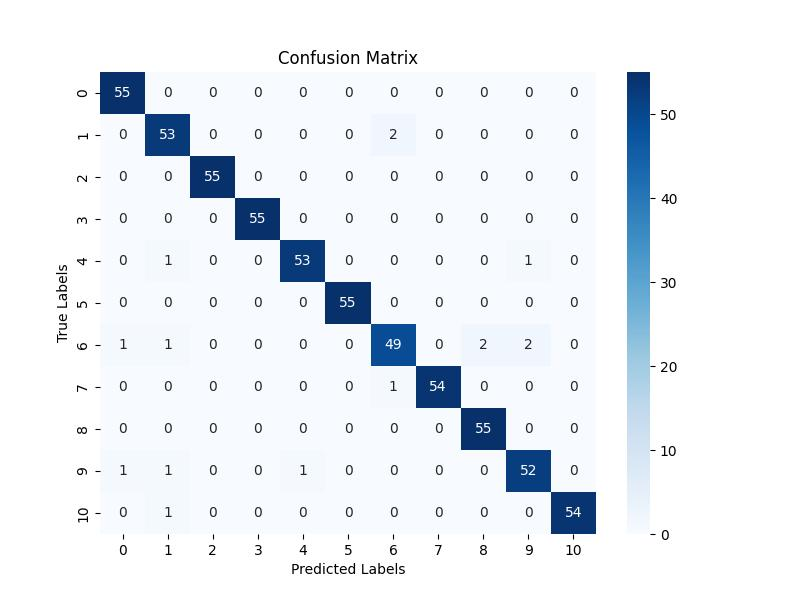
\includegraphics[width=1\linewidth]{confusion_matrix.jpg}
\caption{Confusion Matrix}
\label{fig:confusion_matrix}
\end{figure}

The training and validation loss curves in Figure \ref{fig:loss_curves} show a steady decrease, indicating good generalization despite the small dataset.

\begin{figure}[h]
\centering
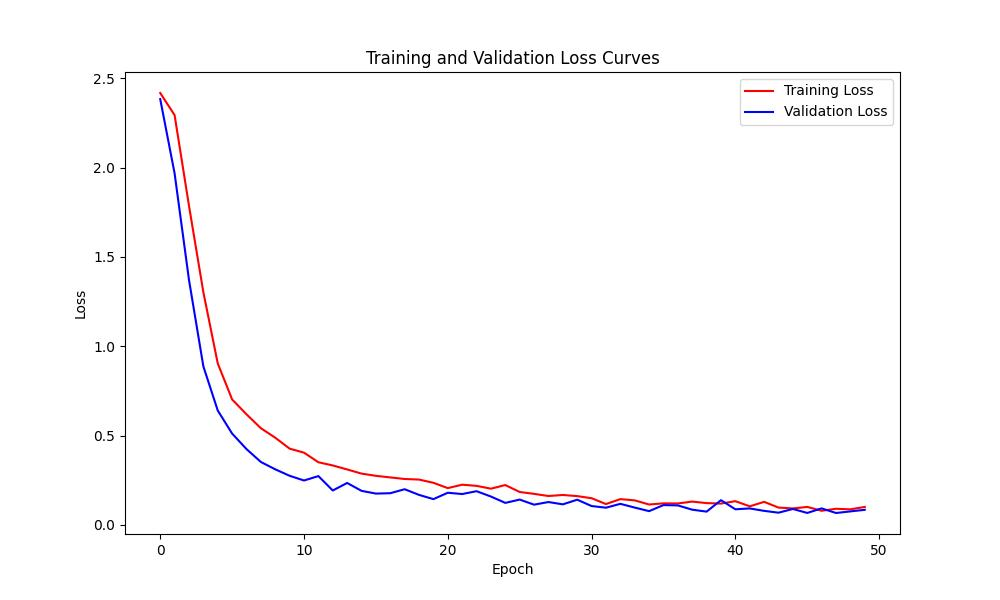
\includegraphics[width=1\linewidth]{loss_curves.jpg}
\caption{Training and Validation Loss Curves}
\label{fig:loss_curves}
\end{figure}

\section{Discussion}
Proposed model demonstrates high precision, recall, and F1-scores, with an overall strong performance. Despite the small dataset size, the model generalizes well, as evidenced by the consistent training and validation loss curves. However, minor misclassifications in similar disease classes suggest that a larger and more diverse dataset could further improve performance. Future work could explore additional augmentation techniques to enhance class separation.

\section{Conclusion}
In this project, I developed the model for automated plant disease identification using Vision Transformers and High-Resolution Networks. The model demonstrated strong performance, suggesting its potential for practical agricultural applications. Future improvements could include training on a larger, more diverse dataset to enhance model robustness.


\bibliographystyle{ieeetr}
\bibliography{ref}

\end{document}
